%%%%%%%%%%%%%%%%%%%%%%%%%%%%%%%%%%%%%%
% LaTeX poster template
% Created by Nathaniel Johnston
% August 2009
% http://www.nathanieljohnston.com/2009/08/latex-poster-template/
%%%%%%%%%%%%%%%%%%%%%%%%%%%%%%%%%%%%%%

\documentclass[final]{beamer}
\usepackage[scale=1.24]{beamerposter}
\usepackage{graphicx}			% allows us to import images
\usepackage[absolute,overlay]{textpos}
\usepackage[labelfont={sf,bf}]{caption}
\usepackage{subfigure}
\usepackage{booktabs}
\usepackage{verbatim}
%\usepackage[utopia]{mathdesign}
%\usepackage[math]{iwona}
%-----------------------------------------------------------
% Define the column width and poster size
% To set effective sepwid, onecolwid and twocolwid values, first choose how many columns you want and how much separation you want between columns
% The separation I chose is 0.024 and I want 4 columns
% Then set onecolwid to be (1-(4+1)*0.024)/4 = 0.22
% Set twocolwid to be 2*onecolwid + sepwid = 0.464
%-----------------------------------------------------------

\newlength{\halfsepwid}
\newlength{\sepwid}
\newlength{\septwowid}
\newlength{\colonewid} % Column 1 width
\newlength{\coltwowid} % Column 2 width
\newlength{\halftwowid} % Half of Col 2
\newlength{\colthreewid}
\newlength{\colfourwid}
\setlength{\paperwidth}{42in}
\setlength{\paperheight}{36in}
\setlength{\halfsepwid}{0.004\paperwidth}
\setlength{\sepwid}{0.6\paperwidth}
\setlength{\septwowid}{0.015\paperwidth}
%\setlength{\colonewid}{0.23\paperwidth}
%\setlength{\coltwowid}{0.35\paperwidth}
\setlength{\colonewid}{0.27\paperwidth}
\setlength{\coltwowid}{0.32\paperwidth}
%\setlength{\halftwowid}{0.19\paperwidth}
\setlength{\colthreewid}{0.33\paperwidth}
\setlength{\colfourwid}{0.1\paperwidth}
\setlength{\topmargin}{-0.75in}
\usetheme{confposter}
\usepackage{exscale}
\usepackage{bm}
%-----------------------------------------------------------
% The next part fixes a problem with figure numbering. Thanks Nishan!
% When including a figure in your poster, be sure that the commands are typed in the following order:
% \begin{figure}
% \includegraphics[...]{...}
% \caption{...}
% \end{figure}
% That is, put the \caption after the \includegraphics
%-----------------------------------------------------------

\usecaptiontemplate{
\small
\structure{\insertcaptionname~\insertcaptionnumber:}
\insertcaption}

\renewcommand{\tablename}{\textbf Table}
\renewcommand{\figurename}{\textbf Figure}

%-----------------------------------------------------------
% Define colours (see beamerthemeconfposter.sty to change these colour definitions)
%-----------------------------------------------------------

\setbeamercolor{block title}{fg=dgreen,bg=white}
\setbeamercolor{block body}{fg=black,bg=white}
\setbeamercolor{block alerted title}{fg=white,bg=dblue!70}
\setbeamercolor{block alerted body}{fg=black,bg=dblue!10}
\setbeamercolor{itemize item}{fg=black}
%%%%%%%%%%%%%%%% ADDITIONAL COMMANDS %%%%%%%%%%%%
\newcommand{\be}{\begin{eqnarray}}
\newcommand{\ee}{\end{eqnarray}}
\newcommand{\bee}{\begin{eqnarray*}}
\newcommand{\eee}{\end{eqnarray*}}

\newcommand{\bi}{\begin{itemize}}
\newcommand{\ei}{\end{itemize}}

\newcommand{\vone}{\vspace{1mm}}
\newcommand{\vtwo}{\vspace{2mm}}
\newcommand{\vthree}{\vspace{3mm}}
\newcommand{\vfour}{\vspace{4mm}}
\newcommand{\vsix}{\vspace{6mm}}
\newcommand{\veight}{\vspace{8mm}}


%-----------------------------------------------------------
% Name and authors of poster/paper/research
%-----------------------------------------------------------
\title{\hspace{-13in}\includegraphics[height=2.5in, width=10in]{head.png} Spectral Clustering of Chinese Herbal Medicine Network}
\author{\hspace{-3in}\Large Guangyu Tong\inst{1}, Liqi Feng\inst{2}\hspace{.75pt} (NetID: gt57, lf109)}
\institute{\hspace{-4in}\inst{1}Department of Sociology \inst{2}Department of Biostatistics \& Bioinformatics}
%-----------------------------------------------------------
% Start the poster itself
%-----------------------------------------------------------

\begin{document}
\begin{frame}[t]
  \begin{columns}[t]							% the [t] option aligns the column's content at the top
    %\begin{column}{\sepwid}\end{column}			% empty spacer column
    \begin{column}{\colonewid}\vskip-3ex
      \begin{block}{Motivation}

       Traditional Chinese Herbal Medicine (TCHM) is effective in treating many diseases. Yet the nature of TCHM is not well-understood. A prescription of TCHM often includes a compound mixture of 3-10 herbal ingredients and its efficacy highly depends on the synergy effect of herbal ingredients. The challenges in understanding the synergy effect of herbal ingredients arouse because of the complicated interrelationship structure.
       	 
      \vskip1ex
       Spectral Clustering is widely used in problem where the data is arranged in a complex and unknown shape (Zelnik-Manor and Perona, 2005). In this project, the interrelationship between different herbal ingredients is investigated by Spectral Clustering. 
	   \bi
        \setlength{\itemindent}{1em}
        	\item \vskip1ex The interrelationship between herbal ingredients is represented by a communication network where ingredients shown on the same prescription are connected;
	       \item \vskip1ex Normalized symmetric graph Laplacian is used to investigate the communication network.
	     \ei

    \end{block}
     \vskip1ex

    \begin{block}{TCHM prescription data}
    \begin{figure}[!htb]
            \caption{Medicine network of $603$ prescriptions from  a THCM text book ($V=213$, $E=2633$). Only degree $>25$ presented.}
            \centering
            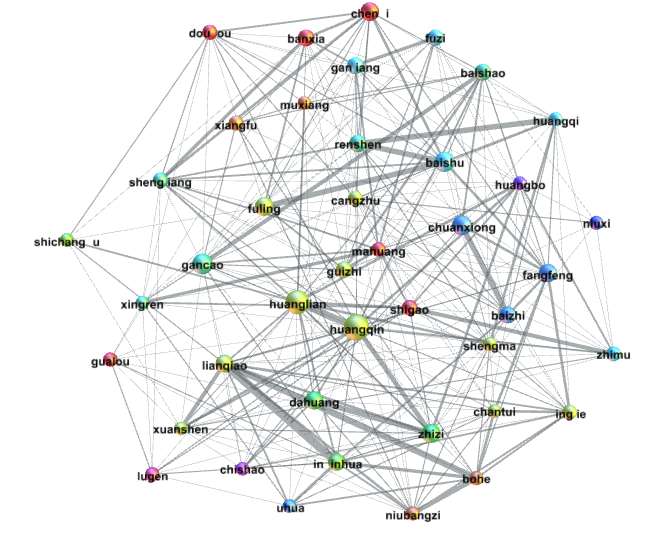
\includegraphics[scale=1.8]{network.png}
        \end{figure}
        \vskip-1ex
    \end{block}


\end{column}

% Column 2
  %\begin{column}{\sepwid}\end{column}			% empty spacer column
    \begin{column}{\coltwowid}
      \begin{alertblock}{Symmetric Graph Laplacian \\Spectral Clustering}
      \bi
      	     \item Weighted {\it adjacency matrix} of a communication network $W=(w_{ij})_{i,j=1,...,n}$ where ingredients $\nu_i$ and $\nu_j$ disconnected $\rightarrow$$w_{ij}=0$. Otherwise, $w_{ij}$ is the number of prescriptions ingredients $\nu_i$ and $\nu_j$ that are both on
	     \item graph Laplacian $L=D-W$ where $D$ is a diagonal degree matrix, $D_{i}=\sum_{j=1}^{n}w_{ij}$
	     \item Herbal ingredients have similar degrees of edges as a prescription often contains a lot of ingredients 
            \item Symmetric graph Laplacian $L_n=D^{-\frac{1}{2}}LD^{-\frac{1}{2}}$
         \ei     
         \vskip1ex
            {\bf Number of clusters is determined by the eigengap heuristic}
           \bi
           	\item The number of small eigenvalues ($\approx 0$) of $L_{sym}$ indicates the number of clusters in the original communication network
		\item Determine the appropriate number of clusters by finding the eigenvalue $\lambda_k$ of of $L_{sym}$ and $\lambda_{k+1}$ is relatively large. k is the number of clusters used in the analysis
           \ei
     
      \end{alertblock}
      \vskip1ex
	
        \begin{block}{Algorithm {\small(Ng, Jordan and Weiss, 2002)}}
      \bi
        \setlength{\itemindent}{1em}
         \item[1)] Construct a similarity graph by connecting two herbal ingredients if they appear on the some description with the weight of edge being the total number of prescriptions they both show up.\vskip1ex
         \item[2)] Compute the normalized Laplacian $L_{sym}$.\vskip1ex
         \item[3)] Compute the first k eigenvectors (ascending order) $u_1, ..., u_k$ of $L_{sym}$.\vskip1ex
         \item[4)] Let $U$ $\in \mathbb{R}^{n\times k}$ contains $u_1, ..., u_k$ as columns. \vskip1ex
         \item[5)] Form the matrix $T \in \mathbb{R}^{n\times k}$ from $U$ by normalizing the rows to norm 1 ($t_{ij}=u_{ij}/(\sum_{k}u_{ik}^{2})^{\frac{1}{2}}$).\vskip1ex
         \item[6)] For $i= 1,...,n$, let $y_i \in \mathbb{R}^k$ be the vector corresponding to the $i^{th}$ row of $T$.\vskip1ex
         \item[7)] Clusters the points $(y_i)_{i=1,...,n}$ with the $k$-nearest neighbor algorithm into clusters $C_1,....,C_k$.
         
      \ei
    \end{block}
    
      \begin{block}{}
    {\tiny The above analysis was done using R (version 3.2.2). Package igraph is employed to construct the communication network and package kknn is used for spectral clustering. Package igraph is used to generate method comparison table.}
    \end{block}
    \end{column}
  

% Column 3
  %\begin{column}{\sepwid}\end{column}			% empty spacer column
  \begin{column}{\colthreewid}\vskip-3ex
    \begin{block}{Results}
    
\begin{figure}[!htb]
           % \caption{Eigenvalue plot of the Laplacian matrices. Two arrows indicate the optimal numbers of clusters for the algorithm}
           %%%%%%%%%%%%%%%%%
           % question: what do you mean by for K=4? I thought K is the number
           % of clusters to be determined from the graph. Here K should be somewhat
           % close to 7 or 14? Am I misunderstanding? If not, delete K, it is confusing 
           % and has nothing to do with the eigenvalues
           %%%%%%%%%%%%%%%%%
           \caption{Eigenvalue plot of the Laplacian matrices. Two arrows indicate the optimal number of cluster for the algorithm (eigengap heuristic)}
            \centering
            \vspace{-1in}
            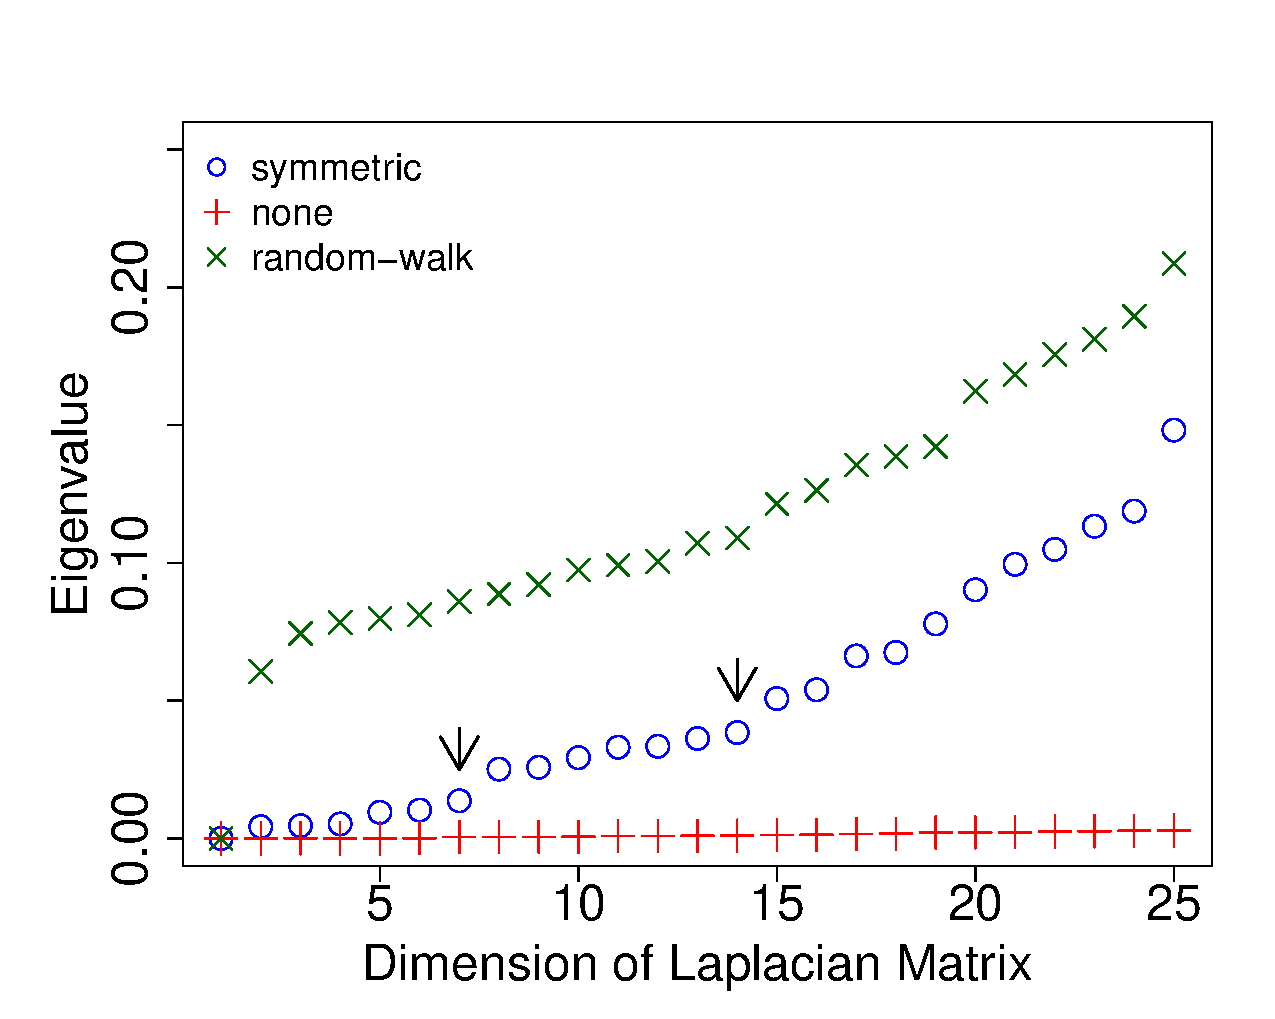
\includegraphics[scale=1.4]{eigenplot.pdf}
        \end{figure}
     
    
    
     \begin{table}[ht]
  \centering
  \caption{Comparison of performance between different clustering methods.}
  \begin{tabular}{llc}
    \toprule
    Method & $\#$ Clusters & Misclassification Rates ($\%$) \\ 
    \midrule
    Lap-Symm & 14 ($K=4$) & ({\color{blue}{14.3}}, 34.2) \\ 
    Lap-Symm & 4 ($K=10$) & (38.8, {\color{blue}{10.0}}) \\ 
    Lap-None & 12 ($K=3$) & (40.0, 36.8) \\ 
    Betweenness & 84 & (8.0, 23.5) \\ 
    InfoMap & 68 & (0.0, 50.0) \\ 
    Label Propogation & 1 & (47.5, 100.0) \\ 
    Lead Eigenvalue & 10 & (13.0, 30.6)\\
    Multilevel & 6 & (13.0, 30.6)\\
    Stat Mechanics & 7 & (13.0, 30.6)\\
    Short Ran-Walk & 14 & (17.9, 25.8)\\
   \bottomrule
\end{tabular}
\end{table}
%% changed part-Liqi
\centering
{\small misclassification rates is computed as the Type I error and Type II error}\\
      \end{block}

 \begin{block}{Conclusion}
      \bi
        \setlength{\itemindent}{1em}
        
        %%%%%%%%%%%%%%%%%%
        % changes made, revert it if you
        % think it does not make sense
        % PS: I change the graph laplacian spectrum->graph laplacian spectral
        %%%%%%%%%%%%%%%%%%
        
       %  \item[1)] Graph Laplacian spectral clustering achieves reliable performance in terms of the both ends of misclassification error rate.\vskip1ex
        \item[1)] Graph Laplacian spectral clustering achieves reliable performance (small Type I and Type II errors).\vskip1ex
         %\item[2)] Graph Laplacian spectral clustering outperforms other methods in terms of the performance of wrong combinations to right.  \vskip1ex
         
         %% somewhat confusing what exactly do you mean-Liqi
         \item[2)] Graph Laplacian spectral clustering outperforms other methods in probing wrong prescription combinations.  \vskip1ex
         
         
         %% method->approach -Liqi
         \item[3)] Symmetric approach outperforms the unnomalized approach and the random walk approach. \vskip1ex
        % \item[4)] Larger dataset and other information, such as diseases, can further improve the performance of this method. \vskip1ex
        \item[4)] The performance of clustering can be improved with a larger sample of prescriptions and disease information. \vskip1ex
      \ei
    \end{block}
    


  \end{column}

\begin{column}{\colfourwid}\vskip-3ex
\qquad
\end{column}	

 \end{columns}
\end{frame}
\end{document}

